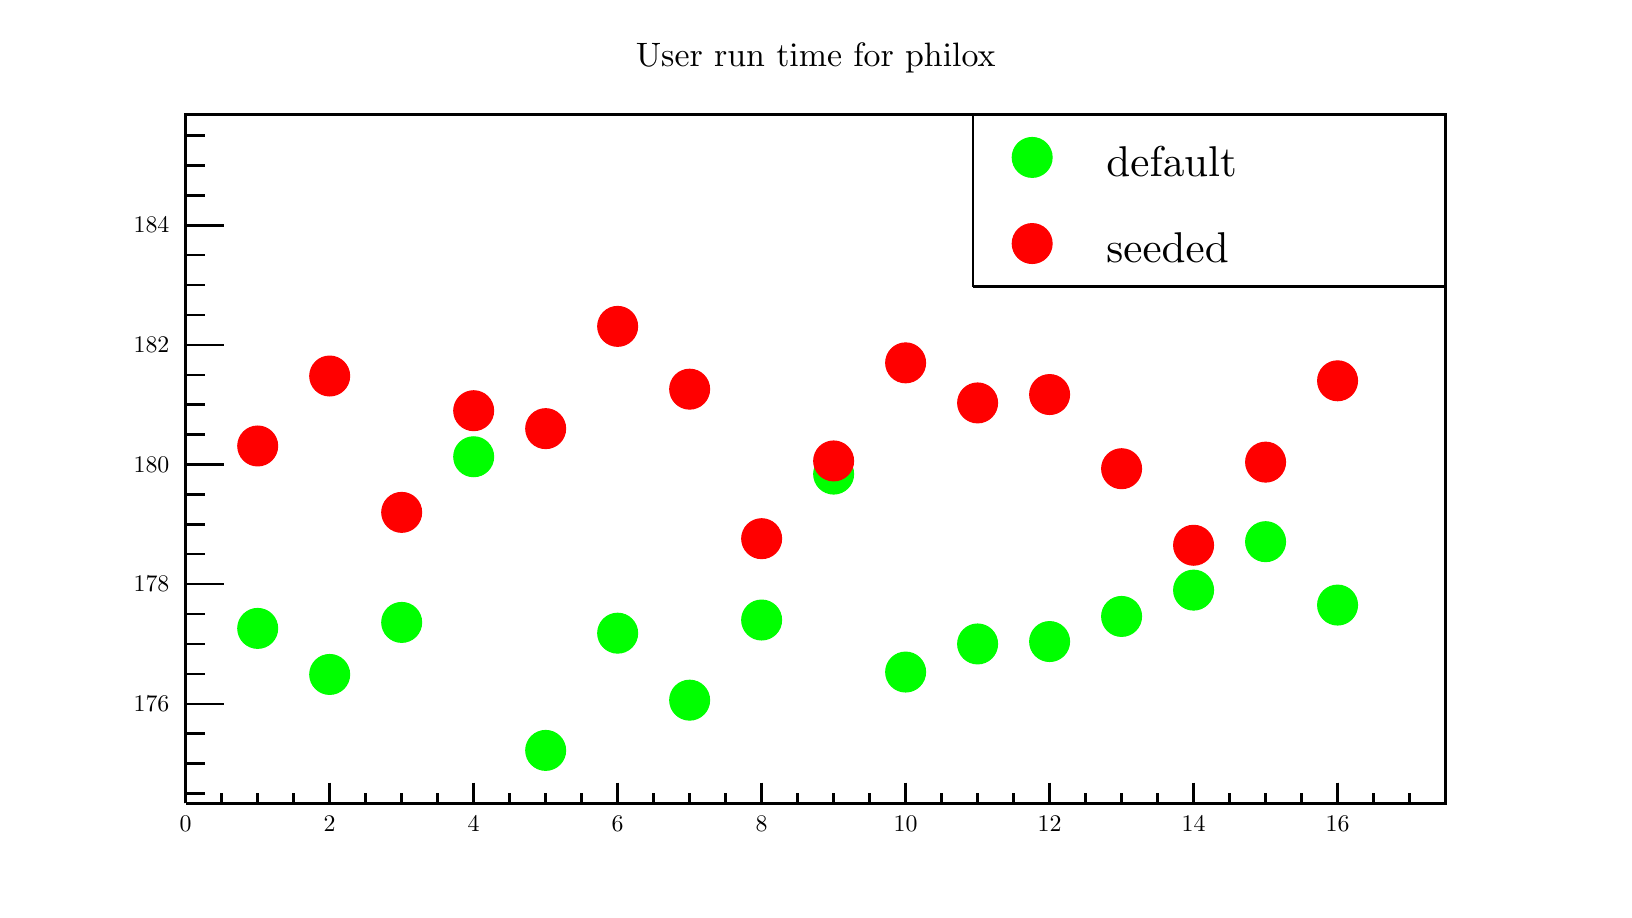
\begin{tikzpicture}
\pgfdeclareplotmark{cross} {
\pgfpathmoveto{\pgfpoint{-0.3\pgfplotmarksize}{\pgfplotmarksize}}
\pgfpathlineto{\pgfpoint{+0.3\pgfplotmarksize}{\pgfplotmarksize}}
\pgfpathlineto{\pgfpoint{+0.3\pgfplotmarksize}{0.3\pgfplotmarksize}}
\pgfpathlineto{\pgfpoint{+1\pgfplotmarksize}{0.3\pgfplotmarksize}}
\pgfpathlineto{\pgfpoint{+1\pgfplotmarksize}{-0.3\pgfplotmarksize}}
\pgfpathlineto{\pgfpoint{+0.3\pgfplotmarksize}{-0.3\pgfplotmarksize}}
\pgfpathlineto{\pgfpoint{+0.3\pgfplotmarksize}{-1.\pgfplotmarksize}}
\pgfpathlineto{\pgfpoint{-0.3\pgfplotmarksize}{-1.\pgfplotmarksize}}
\pgfpathlineto{\pgfpoint{-0.3\pgfplotmarksize}{-0.3\pgfplotmarksize}}
\pgfpathlineto{\pgfpoint{-1.\pgfplotmarksize}{-0.3\pgfplotmarksize}}
\pgfpathlineto{\pgfpoint{-1.\pgfplotmarksize}{0.3\pgfplotmarksize}}
\pgfpathlineto{\pgfpoint{-0.3\pgfplotmarksize}{0.3\pgfplotmarksize}}
\pgfpathclose
\pgfusepathqstroke
}
\pgfdeclareplotmark{cross*} {
\pgfpathmoveto{\pgfpoint{-0.3\pgfplotmarksize}{\pgfplotmarksize}}
\pgfpathlineto{\pgfpoint{+0.3\pgfplotmarksize}{\pgfplotmarksize}}
\pgfpathlineto{\pgfpoint{+0.3\pgfplotmarksize}{0.3\pgfplotmarksize}}
\pgfpathlineto{\pgfpoint{+1\pgfplotmarksize}{0.3\pgfplotmarksize}}
\pgfpathlineto{\pgfpoint{+1\pgfplotmarksize}{-0.3\pgfplotmarksize}}
\pgfpathlineto{\pgfpoint{+0.3\pgfplotmarksize}{-0.3\pgfplotmarksize}}
\pgfpathlineto{\pgfpoint{+0.3\pgfplotmarksize}{-1.\pgfplotmarksize}}
\pgfpathlineto{\pgfpoint{-0.3\pgfplotmarksize}{-1.\pgfplotmarksize}}
\pgfpathlineto{\pgfpoint{-0.3\pgfplotmarksize}{-0.3\pgfplotmarksize}}
\pgfpathlineto{\pgfpoint{-1.\pgfplotmarksize}{-0.3\pgfplotmarksize}}
\pgfpathlineto{\pgfpoint{-1.\pgfplotmarksize}{0.3\pgfplotmarksize}}
\pgfpathlineto{\pgfpoint{-0.3\pgfplotmarksize}{0.3\pgfplotmarksize}}
\pgfpathclose
\pgfusepathqfillstroke
}
\pgfdeclareplotmark{newstar} {
\pgfpathmoveto{\pgfqpoint{0pt}{\pgfplotmarksize}}
\pgfpathlineto{\pgfqpointpolar{44}{0.5\pgfplotmarksize}}
\pgfpathlineto{\pgfqpointpolar{18}{\pgfplotmarksize}}
\pgfpathlineto{\pgfqpointpolar{-20}{0.5\pgfplotmarksize}}
\pgfpathlineto{\pgfqpointpolar{-54}{\pgfplotmarksize}}
\pgfpathlineto{\pgfqpointpolar{-90}{0.5\pgfplotmarksize}}
\pgfpathlineto{\pgfqpointpolar{234}{\pgfplotmarksize}}
\pgfpathlineto{\pgfqpointpolar{198}{0.5\pgfplotmarksize}}
\pgfpathlineto{\pgfqpointpolar{162}{\pgfplotmarksize}}
\pgfpathlineto{\pgfqpointpolar{134}{0.5\pgfplotmarksize}}
\pgfpathclose
\pgfusepathqstroke
}
\pgfdeclareplotmark{newstar*} {
\pgfpathmoveto{\pgfqpoint{0pt}{\pgfplotmarksize}}
\pgfpathlineto{\pgfqpointpolar{44}{0.5\pgfplotmarksize}}
\pgfpathlineto{\pgfqpointpolar{18}{\pgfplotmarksize}}
\pgfpathlineto{\pgfqpointpolar{-20}{0.5\pgfplotmarksize}}
\pgfpathlineto{\pgfqpointpolar{-54}{\pgfplotmarksize}}
\pgfpathlineto{\pgfqpointpolar{-90}{0.5\pgfplotmarksize}}
\pgfpathlineto{\pgfqpointpolar{234}{\pgfplotmarksize}}
\pgfpathlineto{\pgfqpointpolar{198}{0.5\pgfplotmarksize}}
\pgfpathlineto{\pgfqpointpolar{162}{\pgfplotmarksize}}
\pgfpathlineto{\pgfqpointpolar{134}{0.5\pgfplotmarksize}}
\pgfpathclose
\pgfusepathqfillstroke
}
\definecolor{c}{rgb}{1,1,1};
\draw [color=c, fill=c] (0,0) rectangle (20,10.9387);
\draw [color=c, fill=c] (2,1.09387) rectangle (18,9.84481);
\definecolor{c}{rgb}{0,0,0};
\draw [c,line width=0.9] (2,1.09387) -- (2,9.84481) -- (18,9.84481) -- (18,1.09387) -- (2,1.09387);
\definecolor{c}{rgb}{1,1,1};
\draw [color=c, fill=c] (2,1.09387) rectangle (18,9.84481);
\definecolor{c}{rgb}{0,0,0};
\draw [c,line width=0.9] (2,1.09387) -- (2,9.84481) -- (18,9.84481) -- (18,1.09387) -- (2,1.09387);
\draw [c,line width=0.9] (2,1.09387) -- (18,1.09387);
\draw [c,line width=0.9] (2,1.3564) -- (2,1.09387);
\draw [c,line width=0.9] (2.45714,1.22513) -- (2.45714,1.09387);
\draw [c,line width=0.9] (2.91429,1.22513) -- (2.91429,1.09387);
\draw [c,line width=0.9] (3.37143,1.22513) -- (3.37143,1.09387);
\draw [c,line width=0.9] (3.82857,1.3564) -- (3.82857,1.09387);
\draw [c,line width=0.9] (4.28571,1.22513) -- (4.28571,1.09387);
\draw [c,line width=0.9] (4.74286,1.22513) -- (4.74286,1.09387);
\draw [c,line width=0.9] (5.2,1.22513) -- (5.2,1.09387);
\draw [c,line width=0.9] (5.65714,1.3564) -- (5.65714,1.09387);
\draw [c,line width=0.9] (6.11429,1.22513) -- (6.11429,1.09387);
\draw [c,line width=0.9] (6.57143,1.22513) -- (6.57143,1.09387);
\draw [c,line width=0.9] (7.02857,1.22513) -- (7.02857,1.09387);
\draw [c,line width=0.9] (7.48571,1.3564) -- (7.48571,1.09387);
\draw [c,line width=0.9] (7.94286,1.22513) -- (7.94286,1.09387);
\draw [c,line width=0.9] (8.4,1.22513) -- (8.4,1.09387);
\draw [c,line width=0.9] (8.85714,1.22513) -- (8.85714,1.09387);
\draw [c,line width=0.9] (9.31429,1.3564) -- (9.31429,1.09387);
\draw [c,line width=0.9] (9.77143,1.22513) -- (9.77143,1.09387);
\draw [c,line width=0.9] (10.2286,1.22513) -- (10.2286,1.09387);
\draw [c,line width=0.9] (10.6857,1.22513) -- (10.6857,1.09387);
\draw [c,line width=0.9] (11.1429,1.3564) -- (11.1429,1.09387);
\draw [c,line width=0.9] (11.6,1.22513) -- (11.6,1.09387);
\draw [c,line width=0.9] (12.0571,1.22513) -- (12.0571,1.09387);
\draw [c,line width=0.9] (12.5143,1.22513) -- (12.5143,1.09387);
\draw [c,line width=0.9] (12.9714,1.3564) -- (12.9714,1.09387);
\draw [c,line width=0.9] (13.4286,1.22513) -- (13.4286,1.09387);
\draw [c,line width=0.9] (13.8857,1.22513) -- (13.8857,1.09387);
\draw [c,line width=0.9] (14.3429,1.22513) -- (14.3429,1.09387);
\draw [c,line width=0.9] (14.8,1.3564) -- (14.8,1.09387);
\draw [c,line width=0.9] (15.2571,1.22513) -- (15.2571,1.09387);
\draw [c,line width=0.9] (15.7143,1.22513) -- (15.7143,1.09387);
\draw [c,line width=0.9] (16.1714,1.22513) -- (16.1714,1.09387);
\draw [c,line width=0.9] (16.6286,1.3564) -- (16.6286,1.09387);
\draw [c,line width=0.9] (16.6286,1.3564) -- (16.6286,1.09387);
\draw [c,line width=0.9] (17.0857,1.22513) -- (17.0857,1.09387);
\draw [c,line width=0.9] (17.5429,1.22513) -- (17.5429,1.09387);
\draw [c,line width=0.9] (18,1.22513) -- (18,1.09387);
\draw [anchor=base] (2,0.732891) node[scale=0.861703, color=c, rotate=0]{0};
\draw [anchor=base] (3.82857,0.732891) node[scale=0.861703, color=c, rotate=0]{2};
\draw [anchor=base] (5.65714,0.732891) node[scale=0.861703, color=c, rotate=0]{4};
\draw [anchor=base] (7.48571,0.732891) node[scale=0.861703, color=c, rotate=0]{6};
\draw [anchor=base] (9.31429,0.732891) node[scale=0.861703, color=c, rotate=0]{8};
\draw [anchor=base] (11.1429,0.732891) node[scale=0.861703, color=c, rotate=0]{10};
\draw [anchor=base] (12.9714,0.732891) node[scale=0.861703, color=c, rotate=0]{12};
\draw [anchor=base] (14.8,0.732891) node[scale=0.861703, color=c, rotate=0]{14};
\draw [anchor=base] (16.6286,0.732891) node[scale=0.861703, color=c, rotate=0]{16};
\draw [c,line width=0.9] (2,1.09387) -- (2,9.84481);
\draw [c,line width=0.9] (2.48,2.35946) -- (2,2.35946);
\draw [c,line width=0.9] (2.24,2.73924) -- (2,2.73924);
\draw [c,line width=0.9] (2.24,3.11901) -- (2,3.11901);
\draw [c,line width=0.9] (2.24,3.49879) -- (2,3.49879);
\draw [c,line width=0.9] (2.48,3.87856) -- (2,3.87856);
\draw [c,line width=0.9] (2.24,4.25833) -- (2,4.25833);
\draw [c,line width=0.9] (2.24,4.63811) -- (2,4.63811);
\draw [c,line width=0.9] (2.24,5.01788) -- (2,5.01788);
\draw [c,line width=0.9] (2.48,5.39765) -- (2,5.39765);
\draw [c,line width=0.9] (2.24,5.77743) -- (2,5.77743);
\draw [c,line width=0.9] (2.24,6.1572) -- (2,6.1572);
\draw [c,line width=0.9] (2.24,6.53698) -- (2,6.53698);
\draw [c,line width=0.9] (2.48,6.91675) -- (2,6.91675);
\draw [c,line width=0.9] (2.24,7.29652) -- (2,7.29652);
\draw [c,line width=0.9] (2.24,7.6763) -- (2,7.6763);
\draw [c,line width=0.9] (2.24,8.05607) -- (2,8.05607);
\draw [c,line width=0.9] (2.48,8.43584) -- (2,8.43584);
\draw [c,line width=0.9] (2.48,2.35946) -- (2,2.35946);
\draw [c,line width=0.9] (2.24,1.97969) -- (2,1.97969);
\draw [c,line width=0.9] (2.24,1.59992) -- (2,1.59992);
\draw [c,line width=0.9] (2.24,1.22014) -- (2,1.22014);
\draw [c,line width=0.9] (2.48,8.43584) -- (2,8.43584);
\draw [c,line width=0.9] (2.24,8.81562) -- (2,8.81562);
\draw [c,line width=0.9] (2.24,9.19539) -- (2,9.19539);
\draw [c,line width=0.9] (2.24,9.57517) -- (2,9.57517);
\draw [anchor= east] (1.9,2.35946) node[scale=0.861703, color=c, rotate=0]{176};
\draw [anchor= east] (1.9,3.87856) node[scale=0.861703, color=c, rotate=0]{178};
\draw [anchor= east] (1.9,5.39765) node[scale=0.861703, color=c, rotate=0]{180};
\draw [anchor= east] (1.9,6.91675) node[scale=0.861703, color=c, rotate=0]{182};
\draw [anchor= east] (1.9,8.43584) node[scale=0.861703, color=c, rotate=0]{184};
\definecolor{c}{rgb}{0,1,0};
\foreach \P in {(2.91429,3.31649), (3.82857,2.73164), (4.74286,3.39245), (5.65714,5.4964), (6.57143,1.76702), (7.48571,3.25573), (8.4,2.40504), (9.31429,3.42283), (10.2286,5.27613), (11.1429,2.76202), (12.0571,3.11901), (12.9714,3.14939),
 (13.8857,3.4684), (14.8,3.8026), (15.7143,4.41784), (16.6286,3.61272)}{\draw[mark options={color=c,fill=c},mark size=7.207207pt,mark=*] plot coordinates {\P};}
\definecolor{c}{rgb}{1,0,0};
\foreach \P in {(2.91429,5.63311), (3.82857,6.52178), (4.74286,4.79002), (5.65714,6.08125), (6.57143,5.85338), (7.48571,7.15221), (8.4,6.35468), (9.31429,4.45582), (10.2286,5.44323), (11.1429,6.68889), (12.0571,6.17999), (12.9714,6.28632),
 (13.8857,5.34449), (14.8,4.37226), (15.7143,5.42804), (16.6286,6.46102)}{\draw[mark options={color=c,fill=c},mark size=7.207207pt,mark=*] plot coordinates {\P};}
\definecolor{c}{rgb}{1,1,1};
\draw [color=c, fill=c] (12,7.65707) rectangle (18,9.84481);
\definecolor{c}{rgb}{0,0,0};
\draw [c,line width=0.9] (12,7.65707) -- (18,7.65707);
\draw [c,line width=0.9] (18,7.65707) -- (18,9.84481);
\draw [c,line width=0.9] (18,9.84481) -- (12,9.84481);
\draw [c,line width=0.9] (12,9.84481) -- (12,7.65707);
\draw [anchor=base west] (13.5,9.05175) node[scale=1.55662, color=c, rotate=0]{default};
\definecolor{c}{rgb}{1,1,1};
\draw [c] (12.225,8.91502) -- (13.275,8.91502) -- (13.275,9.68073) -- (12.225,9.68073);
\draw [c,line width=0.9] (12.225,9.29787) -- (13.275,9.29787);
\definecolor{c}{rgb}{0,1,0};
\foreach \P in {(12.75,9.29787)}{\draw[mark options={color=c,fill=c},mark size=7.207207pt,mark=*] plot coordinates {\P};}
\definecolor{c}{rgb}{0,0,0};
\draw [anchor=base west] (13.5,7.95788) node[scale=1.55662, color=c, rotate=0]{seeded};
\definecolor{c}{rgb}{1,1,1};
\draw [c] (12.225,7.82115) -- (13.275,7.82115) -- (13.275,8.58686) -- (12.225,8.58686);
\draw [c,line width=0.9] (12.225,8.204) -- (13.275,8.204);
\definecolor{c}{rgb}{1,0,0};
\foreach \P in {(12.75,8.204)}{\draw[mark options={color=c,fill=c},mark size=7.207207pt,mark=*] plot coordinates {\P};}
\definecolor{c}{rgb}{0,0,0};
\draw (10,10.5611) node[scale=1.22306, color=c, rotate=0]{User run time for philox};
\end{tikzpicture}
